\documentclass[a4paper, 12pt]{article}

\input{~/Desktop/Studia/LaTeX/setup.tex}
\usepackage{amsmath}


\author{Wojciech Orłowski}
\date{\today}
\title{\textsc{Monte Carlo: symulacja dynamiki gazu}\\ - sprawozdanie}

\begin{document}
	\maketitle

	\section*{Wstęp}
	
	Podczas zajęć wykonano symulacje gazu, którego cząsteczki składają się z jednego atomu.
	Wykorzystano metodę DSMC (Direct Simulation Monte Carlo).
	Metoda ta służy do obliczania już większych układów, zawierających sporą ilość cząsteczek i w tym celu została ona odpowiednio zoptymalizowana.
	Dlatego skorzystano z gotowej klasy, przedstawionej przez prowadzącego, która zawiera odpowiednią implementację.
	W metodzie tej nie uwzględnia się oddziaływania między cząstkami poza ich zderzeniami.
	
	\subsection*{Zderzenia}
	
	W algorytmie zderzenia są wykrywane używając pewnego efektywnego promienia cząstki.
	Prawdopodobieństwo zderzenia zależy też od wektorów prędkości cząsteczek - jest ono zerowe, jeżeli obie cząstki poruszają się w tą samą stronę.
	W celu optymalizacji nie sprawdza się możliwości zderzenia pomiędzy wszystkimi cząstkami.
	Cały obszar obliczeniowy dzielony jest na komórki, a cząstka może się zderzyć z cząsteczki z aktualnej lub granicznej komórki.
	Taki zastosowanie znacznie przyspiesza czas obliczeń.
	Kąt pod jakim są odbijane cząstki też nie jest dokładnie znany i jest losowany.
	Symulacja zderzeń cząsteczek jest najbardziej wymagającym obliczeniowo aspektem całej symulacji.
	
	\subsection*{Warunki początkowe}
	
	Warunki początkowe mogą być różne. 
	W zasadzie chodzi o początkowe ułożenie cząsteczek oraz ich prędkości.
	W klasie możemy nadać kilka różnych warunków początkowych, jeżeli chodzi o ułożenie cząsteczek.
	Warunkiem początkowym prędkości natomiast jest rozkład Maxwella dwuwymiarowy dla danej temperatury początkowej układu.
	Zaczynając od rozkładu Boltzmanna (w zależności od energii) można przejść do prędkościowego rozkładu dla prędkości w dwóch niezależnych kierunkach \eqref{v_rozklad}.
	\begin{equation}
		f_E(v_x,v_y) = \left( \frac{m}{2\pi k_B T} \right) ^ {1/2} \exp(-\frac{mv_x^2}{2k_B T}) \cdot \left( \frac{m}{2\pi k_B T} \right) ^ {1/2} \exp(-\frac{mv_y^2}{2k_B T}) = f_{Ex} \cdot f_{Ey}. 
		\label{v_rozklad}
	\end{equation}
	Zatem składowe prędkości w obu kierunkach są najzwyczajniej losowane z rozkładu normalnego z $\sigma = \sqrt{\frac{k_BT}{m}}$. 
	Aby otrzymać rozkład od wartości prędkości należy dokonać transformacji \eqref{trans}.
	\begin{equation}
		f_E(v_x,v_y)\dd v_x \dd v_y  = 2\pi f_2(v)dv = f_v(v)dv,
		\label{trans}
	\end{equation}
	co w ostateczności daje rozkład \eqref{final}
	\begin{equation}
		f_v(v) = \frac{mv}{k_B T}\exp(\frac{-mv^2}{2k_BT}).
		\label{final}
	\end{equation}
	Takiego rozkładu (z odpowiednim warunkiem normalizacji) można się spodziewać w stanie ustalonym układu, w przypadku stałej temperatury, co wymaga nałożenia odpowiednich warunków brzegowych.
	
	\subsection*{Warunki brzegowe}
	
	Na ściankach cząstki mogą się zachowywać w różny sposób.
	Dla warunku brzegowego Neumanna cząstka jest odbijana od brzegu (nic się z nią nie dzieje), ma to odzwierciedlać zerowanie się pochodnej na brzegu.
	W warunku Dirichleta, na brzeg jest nałożona konkretna temperatura. 
	Zderzenie cząstki z ścianką spowoduje usunięcie jej oraz powstanie nowej cząstki o prędkości wygenerowanej zgodnie z rozkładem Maxwella o temperaturze ścianki.
	
	\subsection*{Krok czasowy}
	
	Ważnym aspektem jest także krok czasowy, gdyż nie jest on stały w trakcie trwania symulacji.
	Wynika to z sprawdzania warunków na odbijanie się cząstek i ograniczenia komórkowego, przez co cząstka nie powinna przekroczyć komórki w trakcie jednego kroku czasowego.
	Zatem na krok czasowy narzucony jest warunek \eqref{timestep}.
	\begin{equation}
		\Delta t (t) \leq \frac{\min(\Delta x, \Delta y)}{V_{max}(t)},
		\label{timestep}
	\end{equation} 
	gdzie $\Delta x, \Delta y$ to rozmiary pojedynczej komórki, na które podzielony jest obszar obliczeniowy.
	
	\section*{Wyniki}
	
	Podczas ćwiczenia skorzystano z klasy przygotowanej przez prowadzącego \texttt{DSMC\_2D}.
	Za jej pomocą przeprowadzono obliczenia wielowątkowe.
	Zrównoleglenie obliczeń znacząco pomogło je przyspieszyć, jednak dla użytej ilości cząstek wciąż były one długie. 
	Stan układu był monitorowany na bieżąco za pomocą rozkładu prędkości cząstek oraz wypluwany na ekran terminala z użyciem \texttt{gnuplota} (opcja \textit{dumb}).
	Przykładowy wykres terminalowy (ASCII) został przedstawiony na rys. \ref{gnuplot_plot} - takie plotowanie wykresów pozwoliło na kontrole obliczeń bez obciążania komputera i przeznaczenie większości jego mocy na faktyczną symulację.
	\begin{figure}[H]
		\centering
		\includegraphics[width=0.6\textwidth]{../plots/gnuplot.png}
		\caption{Wykres drukowany na bieżąco w terminalu w celu kontroli obliczeń.}
		\label{gnuplot_plot}
	\end{figure} 
	
	\noindent W każdym z wykonywanych przykładów ustawiono następujące parametry
	\begin{itemize}
		\item liczba cząsteczek = 10000;
		\item liczba typów cząsteczek = 1;
		\item masa jednej cząsteczki = $40\cdot10^{-27}$ kg;
		\item rozmiary obszaru = [0,1] x [0,1];
		\item stała Boltzmanna 1.38$\cdot10^{-23}$
		\item $nx = 50 \; \; \; ny = 50$;
		\item temperatura początkowa = 300 K;
	\end{itemize}
	Pozostałe parametry dotyczące ułożenia początkowego cząsteczek oraz warunków brzegowych były zmieniane w zależności od zadania.
	Ponadto każde z zadań wykonano dla dwóch rozmiarów cząstek $r = 10^{-6}$ m oraz $r = 10^{-5}$ m.
	
	\subsection*{Zadanie 1}
	
	W pierwszym zadaniu ustawiono parametr \texttt{init\_dist} na 1. 
	Ma to odzwierciedlać sytuacje w której wszystkie cząsteczki początkowo mają identyczną energię oraz identyczne prędkości.
	Warunki brzegowe ustawiono na ściany odbijające (tzn. warunki brzegowe Neumanna).
	O układzie i symulacji uzyskujemy dużo informacji, jednak najważniejszą w tym przypadku jest porównanie rozkładów prędkości, gdyż na początku wszystkie cząstki miały jednakową prędkość.
	Rozkłady prędkości dla symulacji z rozmiarami cząstek $r = 10^{-6}$ oraz $r = 10^{-5}$ zostały przedstawione kolejno na rys. \ref{hist_task_1} oraz \ref{hist_task_2}.
	\begin{figure}[H]
		\centering
		\includegraphics[width=\textwidth]{../plots/task_1/hists.pdf}
		\caption{Rozkłady prędkości w trakcie trwania symulacji dla cząstek o promieniu $r = 10^{-6}$.}
		\label{hist_task_1}
	\end{figure}
	
	\noindent Można zauważyć, że duża ilość cząsteczek ma prędkość lekko mniejszą od 500 m/s. 
	Zapewne była to prędkość początkowa cząsteczek.
	Z układ się stabilizował, a pik występowania cząsteczek o tej prędkości malał, aż w końcu osiągnął wartość ustaloną.
	Układ stabilizował się wolno, aż po wielu iteracjach osiągnął wartość stabilną, bardzo zbliżoną do dokładnego rozkładu Maxwella 2D.
	Wartości rozkładu prędkości wciąż delikatnie oscylowały wokół wartości teoretycznej i dokładnej, jednak jest to układ dynamiczny z możliwie za małą ilością cząsteczek.
	Zwiększenie ilości cząsteczek mogłoby spowodować lepsze dopasowanie po ustaleniu, jednak wymagałoby dużo większej mocy obliczeniowej.
	
	\begin{figure}[H]
		\centering
		\includegraphics[width=\textwidth]{../plots/task_2/hists.pdf}
		\caption{Rozkłady prędkości w trakcie trwania symulacji dla cząstek o promieniu $r = 10^{-5}$.}
		\label{hist_task_2}
	\end{figure} 
	
	\noindent W przypadku większego rozmiaru cząsteczek można stwierdzić podobne wnioski.
	Największą różnicą jest dużo szybsze tempo stabilizacji układu.
	Już dla dwusetnej iteracji rozkład prędkości bardzo przypomina rozkład Maxwella.
	Jest on wciąż lekko przesunięty, jednak nie ma dużych pików dla konkretnej prędkości. 
	Dla maksymalnej ilości iteracji (20000) rozkład bardzo przypomina rozkład Maxwella, a różnice są bardzo małe.
	
	\newpage
	
	\subsection*{Zadanie 2}
	
	W drugim zadaniu ustawiono wartość parametru \texttt{init\_dist} na 3.
	Ma te ustawienie oznaczać, że początkowo wszystkie cząstki są umieszczone w jednej komórce.
	Gdy wszystkie cząstki są w jednej komórce rozważana jest duża ilość zderzeń, przez co początkowo jedna iteracja trwa bardzo dużo czasu. 
	Rozkłady położeń cząstek dla obu rozmiarów cząstek zostały przedstawione na rys. \ref{loc_task_3} i \ref{loc_task_4}.
	
	\begin{figure}[H]
		\centering
		\includegraphics[width=\textwidth]{../plots/task_3/evol.pdf}
		\caption{Rozkład cząsteczek wraz z trwaniem symulacji dla cząsteczek o promieniu r = $10^{-6}$.}
		\label{loc_task_3}
	\end{figure}

	\noindent Cząstki początkowo były ciasno zlokalizowane wokół punktu (0,0).
	Następnie ich \textit{fala} propagowała się w układzie. 
	Na podstawie powyższych rysunków można zauważyć miejsca o wyższych stężeniach cząstek.
	Cząsteczki szybko zajmują cały obszar obliczeniowy, jednak nie są równomiernie rozłożone, zarówno w prędkości jak i w położeniu.
	\\
	\\
	W przypadku cząsteczek o większym promieniu (rys. \ref{loc_task_4}) nie zauważamy widocznego obszaru o większym stężeniu cząstek.
	Może to wynikać z faktu, że większe cząsteczki ulegały częściej zderzeniom, przez co się efektywniej rozszerzały.
	W podobnym tempie cząsteczki zajmowały przestrzeń. 
	\begin{figure}[H]
		\centering
		\includegraphics[width=\textwidth]{../plots/task_4/evol.pdf}
		\caption{Rozkład cząsteczek wraz z trwaniem symulacji dla cząsteczek o promieniu r = $10^{-5}$.}
		\label{loc_task_4}
	\end{figure}
	
	\newpage
	
	\subsection*{Zadanie 3}
	
	W trzecim zadaniu nałożono na jedną ze ścianek warunek brzegowy Dirichleta, to znaczy miała ona pewną stałą temperaturę, równą 1000 K. 
	Parametr \texttt{init\_dist} ustawiono na 2, co ma oznaczać rozkład Maxwella w całym obszarze.
	Rozkłady temperatury i ciśnienia wzdłuż kierunku $x$ zostały przedstawione na rys. \ref{pt_t5} oraz \ref{pt_t6}.
	
	\begin{figure}[H]
		\centering
		\includegraphics[width = \textwidth]{../plots/task_5/task_5pt.pdf}
		\caption{Rozkład temperatury i ciśnienia wzdłuż kierunku $x$ w czasie trwania symulacji dla cząsteczek o promieniu $r=10^{-6}$.}
		\label{pt_t5}
	\end{figure}

	\noindent Dla obu rozmiarów cząstek temperatura i ciśnienie zachowują się podobnie w czasie.
	Początkowo wyższa temperatura jest bliżej lewego brzegu - czyli tam gdzie ustalono warunek brzegowy Dirichleta o wartości 1000 K. 
	Wartość ta jednak nie jest równa 1000 K w początkowych iteracjach, co oznacza, że układ powoli się stabilizuje. 
	Po stabilizacji temperatura jest jednakowa w całym układzie i wynosi około 1000 K. 
	Jest to logiczne, gdyż ściankę traktujemy jako otoczenie, którego temperatura się nie zmienia. 
	\\
	\\
	Można też zauważyć korelację między wartościami temperatury, a wartościami ciśnienia.
	W obszarach o wyższej temperaturze wyższe jest też ciśnienie. 
	Obszary te są obszarami o stałej objętości, więc zależność tą można wytłumaczyć korzystając np. z równania Clapeyrona 
	\[ pV = nRT. \]
	Dla cząsteczek o większym promieniu można stwierdzić podobne wnioski.
	Tempo stabilizacji jest podobne, czyli w każdej iteracji podobna ilość cząstek zderza się z lewą ścianką. 
	
	\begin{figure}[H]
		\centering
		\includegraphics[width = \textwidth]{../plots/task_6/task_6pt.pdf}
		\caption{Rozkład temperatury i ciśnienia wzdłuż kierunku $x$ w czasie trwania symulacji dla cząsteczek o promieniu $r=10^{-5}$.}
		\label{pt_t6}
	\end{figure}
	
	\noindent Rozkłady prędkości dla obu rozmiarów cząstek zostały przedstawione na rys. \ref{hist_task_56}.
	\begin{figure}[H]
		\centering
		\begin{subfigure}{0.49\textwidth}
			\centering
			\includegraphics[width=\textwidth]{../plots/task_5/task_5hists.pdf}
			\caption{}
		\end{subfigure}
		\begin{subfigure}{0.49\textwidth}
			\centering
			\includegraphics[width=\textwidth]{../plots/task_6/task_6hists.pdf}
			\caption{}
		\end{subfigure}
		\caption{Początkowe i końcowe rozkłady prędkości dla cząstek o rozmiarze (a) $r = 10^{-6}$, (b) $r = 10^{-5}$.}
		\label{hist_task_56}
	\end{figure}
	
	\noindent Dla obu przypadków uzyskano podobne wyniki. 
	Oba rozkłady początkowy i są rozkładami Maxwella 2D, a przynajmniej rozkładami do niego zbliżonymi.
	Początkowy jest rozkładem dla temperatury początkowej 300 K, a końcowy dla temperatury końcowej 1000 K.
	Pewnym błędem jest wciąż duża ilość cząstek w układzie o dużej prędkości pod koniec trwania symulacji.
	Może to wynikać ze sposobu losowania nowych cząsteczek na lewym brzegu. 
	
	\subsection*{Zadanie 4}
	
	Ustalono na prawym brzegu także warunek Dirichleta, o wartości temperatury 300 K.
	Przestrzenne rozkłady temperatury i ciśnienia zostały przedstawione na rys. \ref{pt_t7} oraz \ref{pt_t8}.
	
	\begin{figure}[H]
		\centering
		\includegraphics[width = \textwidth]{../plots/task_7/task_7pt.pdf}
		\caption{Rozkład temperatury i ciśnienia wzdłuż kierunku $x$ w czasie trwania symulacji dla cząsteczek o promieniu $r=10^{-6}$.}
		\label{pt_t7}
	\end{figure}
	
	\noindent Ponownie ciężko jest zauważyć większe różnice na symulacjach z różnym rozmiarem cząstek.
	Początkowo rozkład temperatur podobny jest do przypadku poprzedniego. 
	Jednak wraz z czasem trwania symulacji temperatura nie ustala wartości w całej obszarze, jednak widzimy jej liniowe zachowanie.
	Przy prawym brzegu jest ona niższa, a prze lewym wyższa, jednak nie są to temperatury brzegowe.
	Możliwe, że układ jeszcze się ustabilizował, jednak aktualne zachowanie jest całkowicie przewidywalne.
	Cząstka, która powstała na lewym brzegu miesza się z cząstkami o mniejszej energii, a cząstka powstała na prawym brzegu miesza się z cząstkami o wyższej energii, tak że nigdy nie zostanie osiągnięty zakres 300 K - 1000 K. 
	\\
	\\
	Już nie można zauważyć takiej korelacji między wartościami ciśnienia i temperatury jak wcześniej. 
	Może to wynikać z właśnie powstałego gradientu temperatur. 
	
	\begin{figure}[H]
		\centering
		\includegraphics[width = \textwidth]{../plots/task_8/task_8pt.pdf}
		\caption{Rozkład temperatury i ciśnienia wzdłuż kierunku $x$ w czasie trwania symulacji dla cząsteczek o promieniu $r=10^{-5}$.}
		\label{pt_t8}
	\end{figure}
	
	\noindent Rozkłady prędkości początkowe i końcowe zostały przedstawione na rys. \ref{hist_task_78}.
	
		\begin{figure}[H]
		\centering
		\begin{subfigure}{0.49\textwidth}
			\centering
			\includegraphics[width=\textwidth]{../plots/task_7/task_7hists.pdf}
			\caption{}
		\end{subfigure}
		\begin{subfigure}{0.49\textwidth}
			\centering
			\includegraphics[width=\textwidth]{../plots/task_8/task_8hists.pdf}
			\caption{}
		\end{subfigure}
		\caption{Początkowe i końcowe rozkłady prędkości dla cząstek o rozmiarze (a) $r = 10^{-6}$, (b) $r = 10^{-5}$.}
		\label{hist_task_78}
	\end{figure}
	
	\noindent Oba rozkłady przypominają rozkład Maxwella 2D. 
	Ponownie dla rozkładu końcowego istnieje pewien pik dla dużych wartości prędkości - często występujące duże prędkości mogą wynikać z ich częstego losowania na ściankach.
	Biorąc pod uwagę, że temperatura nie ma jednej wartości w badanym obszarze rozkład końcowy jest pewnie rozkładem mieszanym po wszystkim występujących temperaturach.
	Między rozkładami nie ma znaczących różnic wynikających z wielkości cząstek.
	
	\section*{Podsumowanie}
	
	Bezpośrednia symulacja cząstek gazu jest ciekawym narzędziem, pozwalającym w szybki sposób oszacować zachowanie się gazu w danych warunkach.
	Pomimo faktycznego długiego czasu potrzebnego na przeprowadzenie symulacji było to możliwe na domowym komputerze w miarę niskim czasie. 
	Biorąc pod uwagę oddziaływania międzyatomowe byłoby to już nie możliwe.
	Duże spowolnienie powodowałby dokładny mechanizm zderzeniowy cząstek. 
	\\
	\\
	W przypadku symulacji o ustalonym zerowym gradiencie temperatury na brzegach (warunki brzegowe Neumanna) wielkość cząsteczek odegrała znaczący wpływ na szybkość ustalania się stanu stabilnego. 
	Już w 200 iteracji dla cząsteczek, których promień był rząd wyższy uzyskano zbieżność. 
	Dla przypadku w którym ustalono na brzegu warunek Dirichleta tempo zbieżności było podobne w obu przypadkach.
	
	
\end{document}